\documentclass[12pt]{article}\usepackage[]{graphicx}\usepackage[]{color}
%% maxwidth is the original width if it is less than linewidth
%% otherwise use linewidth (to make sure the graphics do not exceed the margin)
\makeatletter
\def\maxwidth{ %
  \ifdim\Gin@nat@width>\linewidth
    \linewidth
  \else
    \Gin@nat@width
  \fi
}
\makeatother

\definecolor{fgcolor}{rgb}{0.345, 0.345, 0.345}
\newcommand{\hlnum}[1]{\textcolor[rgb]{0.686,0.059,0.569}{#1}}%
\newcommand{\hlstr}[1]{\textcolor[rgb]{0.192,0.494,0.8}{#1}}%
\newcommand{\hlcom}[1]{\textcolor[rgb]{0.678,0.584,0.686}{\textit{#1}}}%
\newcommand{\hlopt}[1]{\textcolor[rgb]{0,0,0}{#1}}%
\newcommand{\hlstd}[1]{\textcolor[rgb]{0.345,0.345,0.345}{#1}}%
\newcommand{\hlkwa}[1]{\textcolor[rgb]{0.161,0.373,0.58}{\textbf{#1}}}%
\newcommand{\hlkwb}[1]{\textcolor[rgb]{0.69,0.353,0.396}{#1}}%
\newcommand{\hlkwc}[1]{\textcolor[rgb]{0.333,0.667,0.333}{#1}}%
\newcommand{\hlkwd}[1]{\textcolor[rgb]{0.737,0.353,0.396}{\textbf{#1}}}%
\let\hlipl\hlkwb

\usepackage{framed}
\makeatletter
\newenvironment{kframe}{%
 \def\at@end@of@kframe{}%
 \ifinner\ifhmode%
  \def\at@end@of@kframe{\end{minipage}}%
  \begin{minipage}{\columnwidth}%
 \fi\fi%
 \def\FrameCommand##1{\hskip\@totalleftmargin \hskip-\fboxsep
 \colorbox{shadecolor}{##1}\hskip-\fboxsep
     % There is no \\@totalrightmargin, so:
     \hskip-\linewidth \hskip-\@totalleftmargin \hskip\columnwidth}%
 \MakeFramed {\advance\hsize-\width
   \@totalleftmargin\z@ \linewidth\hsize
   \@setminipage}}%
 {\par\unskip\endMakeFramed%
 \at@end@of@kframe}
\makeatother

\definecolor{shadecolor}{rgb}{.97, .97, .97}
\definecolor{messagecolor}{rgb}{0, 0, 0}
\definecolor{warningcolor}{rgb}{1, 0, 1}
\definecolor{errorcolor}{rgb}{1, 0, 0}
\newenvironment{knitrout}{}{} % an empty environment to be redefined in TeX

\usepackage{alltt}

%% page layout
\textheight 9in 
\textwidth 6.5in
\topmargin -0.5in
\oddsidemargin 0in
\evensidemargin 0in
%\hoffset=-0.5in
\voffset=-0.25in

%% packages
\usepackage{scrtime} % for \thistime (this package MUST be listed first!)
\usepackage{amsmath} % essential for cases environment
\usepackage{amsthm} % for theorems and proofs
\usepackage{amsfonts} % mathbb
\usepackage{graphics,graphicx}
\usepackage{multirow} % fancy tables
\usepackage{wasysym} % circle symbols (including half-filled circles)
\usepackage{enumerate} % fancier enumeration (e.g., a,b,c, ...)
%\usepackage{xcolor}
\usepackage{color}
\newcommand{\de}[1]{{\color{red}{\bfseries DE:} #1}}

%% for solutions to multiple choice questions:
\newcommand{\correct}{{\color{blue}\fbox{\color{red}\checkmark} }}

%% macros
\newcommand{\reals}{\mathbb{R}}
\newcommand{\term}[1]{{\bfseries\slshape #1}}
\newcommand{\Ker}{{\text{Ker}\,}}
\newcommand{\Range}{{\text{Range}\,}}
\newcommand{\diag}{{\text{diag}}}
\newcommand{\alg}{{\text{alg}}}
\newcommand{\geom}{{\text{geom}}}
\newcommand{\norm}[1]{\left\|#1\right\|}
\newcommand{\abs}[1]{\left|#1\right|}
\newcommand{\R}{{\cal R}}
\newcommand{\G}{{\cal G}}
\newcommand{\eps}{\varepsilon}
\newcommand{\B}{\cal B}
\newcommand{\Tinf}{T_\textrm{inf}}
\newcommand{\Shat}{{\hat{S}}}
\newcommand{\Ihat}{{\hat{I}}}
\newcommand{\ie}{\emph{i.e., }}
\newcommand{\eg}{\emph{e.g., }}
\newcommand{\Rlogo}{\protect
\includegraphics[height=2ex,keepaspectratio]{images/Rlogo.pdf}\xspace}
\newcommand{\XPPAUT}{\texttt{XPPAUT}\xspace}
\newcommand{\etal}{\textit{et al}.\xspace}
\newcommand\emphblue[1]{\emph{\color{blue}#1}}

%%%%%%%%%%%%%%%%%%%%%%%%%%%%
%% from feverpreamble.tex %%
%%%%%%%%%%%%%%%%%%%%%%%%%%%%

\usepackage{amssymb,latexsym,amsmath,setspace}
%%\usepackage[colorlinks,linkcolor=blue]{hyperref}
\usepackage[colorlinks=true,allcolors=blue]{hyperref}
%%\usepackage[colorlinks]{hyperref}
\usepackage{xspace}
\usepackage{graphics,graphicx}
\usepackage{subfigure}
\usepackage{lineno}
\usepackage{fancyhdr}
\usepackage[english]{babel}  %% for texi2dvi ~ bug
\usepackage[normalem]{ulem}
\usepackage{tikz} % http://www.texample.net/tikz/examples/tikzdevice-demo/
  % N.B. version 0.6.3 of tikzDevice from Rforge is required!!
%% improve figure caption typsetting:  (see ~/tex/caption.pdf for manual)
\usepackage[footnotesize,bf]{caption}
\usepackage{placeins} % \FloatBarrier

% citation macros
\newcommand{\citen}[1]{\cite{#1}}

% comment macros
\usepackage{color}
\newcommand{\comment}[3]{\textcolor{#1}{\textbf{[#2: }\textit{#3}\textbf{]}}}
\newcommand{\david}[1]{\comment{blue}{DE}{#1}}
\newcommand{\paul}[1]{\comment{cyan}{PA}{#1}}
\newcommand{\ben}[1]{\comment{magenta}{BB}{#1}}
\newcommand{\needref}{{\textcolor{red}{[NEED REF]}}}
\newcommand{\TBD}{{\textcolor{red}{{\bf TBD}}}}
% remove comments
%\renewcommand{\comment}[3]{\relax}
% remove section headings
%\def\subsubsection*#1{\relax\nobreak}

% other macros
\newcommand{\avg}[1]{{\left\langle#1\right\rangle}}
\newcommand{\var}[1]{\textrm{var}\left(#1\right)}
\newcommand{\sem}[1]{\textrm{sem}\left(#1\right)}
\newcommand{\natinf}{{\mathcal I}}
\newcommand{\find}{f_{\textrm{i}}}
\newcommand{\fpop}{f_{\textrm{p}}}
\newcommand{\logit}{\textrm{logit}}
\newcommand{\sign}{\textrm{sign}}
\newcommand{\logistic}{\textrm{logistic}}
\def\AJE{{\it American Journal of Epidemiology\/}}
\newcommand{\code}[1]{{\tt #1}}
\newcommand{\magcode}[1]{{\tt\color{magenta}#1}}
\newcommand{\redcode}[1]{{\tt\color{red}#1}}
\newcommand{\blackcode}[1]{{\tt\color{black}#1}}

%%%%%%%%%%%%%%%%%%%
%% JOURNAL NAMES %%
%%%%%%%%%%%%%%%%%%%
\def\PNAS{PNAS}
\def\JAMA{JAMA}
\def\BMB{{\it Bulletin of Mathematical Biology\/}}

% references
\newcommand{\eref}[1]{Equation~\eqref{E:#1}}
\newcommand{\fref}[1]{Figure~\ref{F:#1}}
\newcommand{\tref}[1]{Table~\ref{T:#1}}
\newcommand{\sref}[1]{\S\ref{S:#1}}
% other macros
\newcommand{{\Reff}}{{\mathcal{R}}_{\rm eff}}
\newcommand{{\Sinit}}{S_{\rm init}}
\newcommand{\supp}{Supplementary Information}
\newcommand{\StoppedHere}{\bigskip\bigskip{\textcolor{red}{\hrule\centerline{\bfseries STOPPED HERE}\hrule}}\bigskip\bigskip}
\newcommand{\colvec}[2]{\begin{pmatrix}#1\\#2\end{pmatrix}}
\newcommand{\diagmat}[3]{\begin{pmatrix}#1&0&0\\0&#2&0\\0&0&#3\end{pmatrix}}

\newcommand{\solution}[1]{{\hfill\break\vspace{-0.5\baselineskip}\break\color{blue}\emph{Solution: }#1}}
\newcommand{\tr}{\text{tr}}

\newcommand{\thickredline}{\bigskip{\color{red}\hrule height 5pt}\bigskip}

%% for assignment 3:
\newtheorem{theorem}{Theorem}
\newtheorem{remark}{Remark}
\newcommand{\openset}{{\mathcal O}}
\newcommand{\C}{{\mathcal C}}

% Journal Names
% -------------
% \def\MNRAS{{\it Mon.\ Not.\ R.\ astr.\ Soc.\/}}
\def\MNRAS{{\it Monthly Notices of the Royal Astronomical Society\/}}
% \def\ApJ{{\it Astrophys.~J.\/}}
\def\ApJ{{\it The Astrophysical Journal\/}}
% \def\Interface{{\it J.\ R.\ Soc.\ Lond.\/ \rm Interface}}
\def\Interface{{\it Journal of the Royal Society of London, \rm Interface}}
% \def\ProcA{{\it Proc.\ R.\ Soc.\ Lond.\/ \rm A}}
\def\ProcA{{\it Proceedings of the Royal Society of London, Series\/ \rm A}}
% \def\ProcB{{\it Proc.\ R.\ Soc.\ Lond.\/ \rm B}}
\def\ProcB{{\it Proceedings of the Royal Society of London, Series\/ \rm B}}
% \def\TransB{{\it Phil.\ Trans.\ R.\ Soc.\ Lond.\/ \rm B}}
\def\TransB{{\it Philosophical Transactions of the Royal Society of London, Series\/ \rm B}}
\def\TREE{{\it Trends in Ecology and Evolution\/}}
% \def\JTB{{\it J.\ theor.\ Biol.\/}}
\def\JTB{{\it Journal of Theoretical Biology\/}}
% \def\BE{{\it Behav.\ Ecol.\/}}
\def\BE{{\it Behavioural Ecology\/}}
% \def\BES{{\it Behav.\ Ecol.\ Sociobiol.\/}}
\def\BES{{\it Behavioural Ecology and Sociobiology\/}}
% \def\BJLS{\it Biol.\ J.\ Linn.\ Soc.\/}}
\def\BJLS{{\it Biological Journal of the Linnean Society\/}}
\def\Nature{{\it Nature\/}}
\def\Science{{\it Science\/}}
\def\Lancet{{\it The Lancet\/}}
\def\LancetID{{\it Lancet Infectious Diseases\/}}
% \def\PNAS{{\it Proc.\ Natl.\ Acad.\ Sci.\ USA}}
\def\PNAS{{\it PNAS -- Proceedings of the National Academy of Sciences of the
U.S.A.}}
\def\PLoSMed{{\it PLoS Medicine\/}}
\def\PLoSCB{{\it PLoS Computational Biology\/}}
\def\EID{{\it Emerging Infectious Diseases\/}}
\def\BMB{{\it Bulletin of Mathematical Biology\/}}
\def\AJE{{\it American Journal of Epidemiology\/}}
\def\TPB{{\it Theoretical Population Biology\/}}
\def\JRSS{{\it Journal of the Royal Statistical Society\/}}
\def\JRSSB{{\it Journal of the Royal Statistical Society Series B\/}}
\def\IRV{{\it Influenza and Other Respiratory Viruses\/}}
\def\JAMA{{\it JAMA -- Journal of the American Medical Association\/}}
\def\JGLR{{\it Journal of Great Lakes Research\/}}
\def\NEJM{{\it New England Journal of Medicine\/}}
\def\JMB{{\it Journal of Mathematical Biology\/}}
\def\Interface{{\it Journal of the Royal Society Interface\/}}
\def\THEE{{\it Theoretical Ecology\/}}
\def\Annals{{\it Annals of Internal Medicine\/}}
\def\PRL{{\it Physical Review Letters\/}}
\def\PRX{{\it Physical Review X\/}}
\def\NAMS{{\it Notices of the American Mathematical Society\/}}

%% underline with smash through:
\newcommand*{\undersmash}[1]{\underline{\smash{#1}}}

%% referring to TeX macros
\newcommand\ttbackslash{{\tt\char`\\}}
\newcommand{\macro}[1]{{\tt\ttbackslash#1}}

%%%%%%%%%%%%%%%%%%%%%%%%%%%%%%%%%%%%%%%%%%%%%%%%%%%%%%%
%% QUESTIONS FOR MATH 4MB/6MB ASSIGNMENT 2.          %%
%% The question texts are used in several documents: %%
%% assignment, solutions, template,                  %%
%% hence it is better to load them from this file.   %%
%%%%%%%%%%%%%%%%%%%%%%%%%%%%%%%%%%%%%%%%%%%%%%%%%%%%%%%

%% \section{Plot P\&I mortality in Philadelphia in 1918}

%%% THIS WOULD BE BETTER IF IIDDA WEREN'T DOWN AT THE MOMENT:
%\item Download the data file from the International Infectious Disease Data Archive (IIDDA).  \emph{Note:} IIDDA is currently accessible only from campus or via a VPN connection.
%\begin{enumerate}[(i)]
%  \item Go to \url{http://iidda-dev.mcmaster.ca}
%  \item Request access.
%  \item After access has been granted, login and find the data file.  You can either navitage via the Mortality category or search for Philadelphia.
%\end{enumerate}

\newcommand{\PhilaDataReceived}{%
Confirm that you have received this data file by e-mail:
$$\texttt{pim\_us\_phila\_city\_1918\_dy.csv}$$
This plain text comma-separated-value file can be examined (if you wish) using any plain text editor, such as {\tt Emacs}.
}

\newcommand{\PhilaDataReadA}{%
Read the data into a data frame in \Rlogo, using the \code{read.csv()} function.  For example, the following chunk of \Rlogo code should work:
}

\newcommand{\PhilaDataReadB}{%
The purpose of the last line of code above is to ensure that \Rlogo encodes character strings such as \texttt{"1918-10-15"} as dates.
}

\newcommand{\PhilaDataReproduceA}{%
Reproduce the Philadelphia 1918 P\&I plot:
}

\newcommand{\PhilaDataReproduceB}{%
You'll need to use functions such as \code{plot()}, \code{points()} and \code{lines()}.  For a comprehensive list of graphics parameters accepted by these functions, enter {\tt ?par} into the Console pane in {\tt RStudio}.  There are multiple ways to produce a graph exactly like the above, but the following steps work:
\begin{itemize}
  \item Use \code{plot()} to draw the box and basic annotation and the grey line.  Suppress labels when doing this (\emph{e.g.,} \code{xlab=""}).  The box type is controlled by the \code{bty} option and the orientation of annotation is controlled by the \code{las} option.
  \item Use \code{points()} to draw the heavy red dots with black borders.  The most elegant way to do this is to set the point character type to 21 (\code{pch=21}) and the point background colour to red (\code{bg="red"}).  Alternatively, you can use \code{points()} twice (first to draw the red dots and then to draw the black circles around them).
  \item Use \code{mtext()} to add the $x$ and $y$ axis labels in the margins of the plot.
\end{itemize}
}

%% \section{Estimate $\R_0$ from the Philadelphia P\&I time series}

\newcommand{\EstimateRna}{%
The observed mortality time series $M(t)$ is certainly not equal to the prevalence $I(t)$ that appears in the SIR model.  Suppose, however, that $I(t) = \eta M(t-\tau)$ for all time (where $\eta$ and $\tau$ are constants), \emph{i.e.,} that the mortality curve is exactly a scaled and translated version of the prevalence curve.  Prove that if both $I$ and $M$ are growing exactly exponentially over some time period then their exponential rates are identical.  Thus, if we compare them during the ``exponential phase'' on a logarithmic scale, then both curves will be perfectly straight with exactly the same slope.
}

\newcommand{\EstimateRnb}{%
Fit a straight line to the part of the Philadelphia 1918 mortality time series that looks straight on a logarithmic scale (and show your result in a plot).  Once you get the hang of it, the easiest way to do this is to use the \code{lm()} function in \Rlogo (lm stands for linear model).  Note that the simplest way to draw a straight line with given slope and intercept is with the \code{abline()} function.  If you find \code{lm()} counter-intutive to understand then experiment with \code{abline()} until your eyes tell you that you have discovered a line that provides a good fit.
}

\newcommand{\EstimateRnc}{%
How is the slope of your fitted line related to the parameters of the SIR model?  (\emph{Hint:} When $I$ is small, $S\simeq1$.) Why do you need an independent measure of the mean infectious period to estimate $\R_0$?  If the mean infectious period is 4 days, what is your estimate of $\R_0$?
}

%% \section{Fit the basic SIR model to the Philadelphia P\&I time series}

\newcommand{\FitSIRa}{%
Install the \code{"deSolve"} package.  This
    is done by typing the following command in the Console pane of
    {\tt RStudio}:
    $$\text{\code{install.packages("deSolve")}}$$
You will then be prompted to choose a mirror site from which to download the package.  It doesn't matter which mirror you choose, but choosing a site in Ontario might save a fraction of a second. \emph{Note:} This is a one-time operation.  You do not want an \code{install.packages()} command inside your solutions code.
}

\newcommand{\FitSIRbIntro}{%
Write an \Rlogo function that plots the solution $I(t)$ of the SIR model for given parameter values ($\R_0$ and $1/\gamma$) and given initial conditions ($S_0,I_0$).  Use the {\tt ode()} function in the {\tt deSolve} package.  A few hints:
}

\newcommand{\FitSIRbii}{%
As an example of defining a function (without getting involved with a differential equation), here is a code chunk that defines a function to plot a sine curve, and then executes the function.  Note that the default min and max $x$ values are set in the parameter list of the function definition, but the max $x$ value is changed when the function is executed:
}

\long\def\FitSIRbiiiA{%
Here's another example.  This time we first define the vector field for a differential equation.  We then use this function inside another function that plots the solution of the associated differential equation.  To understand the construction, you can, as usual, study the help page for the calling function (\code{?ode} in this case), but the most important issues are the following.

One of the arguments of the \code{ode()} function is the function that evaluates the vector field at the current time.  To avoid confusion, choose the arguments of your vector field function to be \code{t}, \code{vars} and \code{parms} (in that order):
\begin{center}
\begin{tabular}{r p{4.25in}}
     \code{t} & The current time, which will be used within the vector field function if the system is non-autonomous. \\
     \code{vars} & A named vector of the variables in the system (\eg $S$, $I$).  The variables, as named vector passed to this function, are used in the code that defines the vector field within the function. \\
     \code{parms} & A named vector of the parameters of the system (\eg $\beta$, $\gamma$).  It is convenient---but not necessary---to specify default values for the parameters.
\end{tabular}
\end{center}

It is strongly recommended that you follow exactly the style below when defining vector fields for differential equations that you wish to solve with the \code{ode()} function.  In particular, the construction ``\code{with(as.list(c(parms,vars)), {...})}'' makes the variables and parameters visible within the section of code between the braces (\code{\{...\}}) without having to refer to the vectors or lists in which they are stored.  For example, the code would be much harder to read if each instance of \code{x} were replaced by \code{vars\$x} and each instance of \code{beta} were replaced by \code{parms\$beta}; this issue becomes extremely important for complicated vector fields.
}

\newcommand{\FitSIRbiiiB}{%
The following function plots a single solution of the ODE for a given initial condition (\code{ic}), integration time (\code{tmax}) and times at which the state is to be returned (\code{times}).  The vector field function is passed as the \code{func} argument and the parameter vector is passed as the \code{parms} argument.  If further arguments are given, they are passed to the \code{lines()} function that draws the solution.
}

\newcommand{\FitSIRbiiiC}{%
Note here that the call to the \code{ode()} function gives the arguments in the default order so they are interpretted correctly.  If we wished to write the arguments in a different order then we would have to be explicit about which argument is which.  For example, if we wanted to list the initial conditions last for some deep reason then we would have to write:
}

\newcommand{\FitSIRc}{%
For $I_0=10^{-3}$ and $S_0=1-I_0$, plot the solutions of the SIR model assuming $1/\gamma=4$ days and $\R_0\in\{1.2,1.5,1.8,2,3,4\}$.  Use the \code{legend()} command to make a legend on the plot that shows which curves correspond to which values of $\R_0$.
}

\newcommand{\FitSIRd}{%
By trial and error, find values of $\R_0$ and $\gamma$ that yield a solution of the SIR model that fits the Philadelphia P\&I times series reasonably well.  You can assess the quality of fit using the Euclidean distance between the model solution and the data.  (\emph{Note:}  The trial and error approach is a valuable exercise, but not a suggestion of a method you would really use in practice.  We'll discuss better methods for fitting ODE models to data later.)
}

%% \section{Executive summary for the Public Health Agency}

\long\def\ExecSumm{%
The Public Health Agency of Canada (PHAC) is revising their pandemic plan and has asked your group to summarize what you learned from analyzing the 1918 Philadelphia P\&I time series.  Besides explaining what inferences you feel you can make from your analysis so far, PHAC wants to know what you would investigate if they were to fund you to continue your work full time for a month.  They want a maximum of one page from your group.

Incidentally, you might be interested to know that rumour has it that all of the members of the pandemic planning committee took Math 2C03 at McMaster University between 1980 and 2003, but they all failed.  Also, when the chair of the committee was recently asked ``What is a differential equation?'' he apparently bent over and vomited (it is hard to know quite what to make of this given that PHAC was investigating a norovirus outbreak at the time).

\smallskip
\noindent{\em\underline{Note}: When submitting your assignment solution, it is imperative that the one-page executive summary be printed on its own page.  To start a new page in \LaTeX, use the \macro{newpage} command.  Also, as usual, your summary should be in 12 point font.  Don't try to cram in as much as possible.  Make that page as clear and concise as you can, so that a public health planner can absorb its content quickly and easily.}
}

%%\bibliographystyle{vancouver}
%%\bibliography{4mba2_2018}


%%%%%%%%%%%%%%%%%%%%%%%%%%%%%%%%%%%
%% FANCY HEADER AND FOOTER STUFF %%
%%%%%%%%%%%%%%%%%%%%%%%%%%%%%%%%%%%
\usepackage{fancyhdr,lastpage}
\pagestyle{fancy}
\fancyhf{} % clear all header and footer parameters
%%%\lhead{Student Name: \theblank{4cm}}
%%%\chead{}
%%%\rhead{Student Number: \theblank{3cm}}
%%%\lfoot{\small\bfseries\ifnum\thepage<\pageref{LastPage}{CONTINUED\\on next page}\else{LAST PAGE}\fi}
\lfoot{}
\cfoot{{\small\bfseries Page \thepage\ of \pageref{LastPage}}}
\rfoot{}
\renewcommand\headrulewidth{0pt} % Removes funny header line
%%%%%%%%%%%%%%%%%%%%%%%%%%%%%%%%%%%
\IfFileExists{upquote.sty}{\usepackage{upquote}}{}
\begin{document}

\begin{center}
{\bf Mathematics 4MB3/6MB3 Mathematical Biology\\
\smallskip
2018 ASSIGNMENT 2}\\
\medskip
\underline{\emph{Group Name}}: \texttt{{\color{blue}The Infective Collective}}\\
\medskip
\underline{\emph{Group Members}}: {\color{blue}Aurora Basinski-Ferris, Michael Chong, Daniel Park, Daniel Presta}
\end{center}

\bigskip
\noindent
This assignment was due in class on \textcolor{red}{\bf Monday 5 February 2018 at 11:30am}.

\section{Plot P\&I mortality in Philadelphia in 1918}

\begin{enumerate}[(a)]

\item \PhilaDataReceived

\item \PhilaDataReadA
\begin{knitrout}
\definecolor{shadecolor}{rgb}{0.969, 0.969, 0.969}\color{fgcolor}\begin{kframe}
\begin{alltt}
\hlstd{datafile} \hlkwb{<-} \hlstr{"pim_us_phila_city_1918_dy.csv"}
\hlstd{philadata} \hlkwb{<-} \hlkwd{read.csv}\hlstd{(datafile)}
\hlstd{philadata}\hlopt{$}\hlstd{date} \hlkwb{<-} \hlkwd{as.Date}\hlstd{(philadata}\hlopt{$}\hlstd{date)}
\end{alltt}
\end{kframe}
\end{knitrout}
\PhilaDataReadB

\item \PhilaDataReproduceA
  {\color{blue} \begin{proof}[Solution]
  {\color{magenta}
\begin{knitrout}
\definecolor{shadecolor}{rgb}{0.969, 0.969, 0.969}\color{fgcolor}\begin{kframe}
\begin{alltt}
\hlcom{## first make the box with no annotation or curves}
\hlkwd{plot}\hlstd{(philadata}\hlopt{$}\hlstd{date, philadata}\hlopt{$}\hlstd{pim,} \hlkwc{type}\hlstd{=}\hlstr{"n"}\hlstd{,}
     \hlkwc{bty}\hlstd{=}\hlstr{"L"}\hlstd{,} \hlcom{# no upper or right box lines}
     \hlkwc{ylim}\hlstd{=}\hlkwd{c}\hlstd{(}\hlnum{0}\hlstd{,}\hlnum{800}\hlstd{),} \hlcom{# axis limits}
     \hlkwc{yaxp}\hlstd{=}\hlkwd{c}\hlstd{(}\hlnum{0}\hlstd{,}\hlnum{800}\hlstd{,}\hlnum{4}\hlstd{),} \hlcom{#first two numbers is coordinates of }
                      \hlcom{#extreme tick marks, third number is num. of marks}
     \hlkwc{xaxt}\hlstd{=}\hlstr{'n'}\hlstd{,} \hlcom{#supress x ticks and labels}
     \hlkwc{xlab}\hlstd{=}\hlstr{""}\hlstd{,}
     \hlkwc{ann}\hlstd{=}\hlnum{FALSE}\hlstd{,} \hlcom{# no axis annotation (i.e., no title or axis labels)}
     \hlkwc{xaxs}\hlstd{=}\hlstr{"i"}\hlstd{,} \hlcom{#first tick on x axis is the y axis}
     \hlkwc{las}\hlstd{=}\hlnum{1} \hlcom{# axis label style: always horizontal}
\hlstd{)}
\hlstd{month} \hlkwb{<-} \hlkwd{c}\hlstd{(}\hlnum{9}\hlstd{,}\hlnum{10}\hlstd{,}\hlnum{11}\hlstd{,}\hlnum{12}\hlstd{)} \hlcom{#want sept, oct, nov, dec labels}
\hlstd{ticks} \hlkwb{<-} \hlkwd{seq}\hlstd{(philadata}\hlopt{$}\hlstd{date[}\hlnum{1}\hlstd{],}
             \hlstd{philadata}\hlopt{$}\hlstd{date[}\hlkwd{length}\hlstd{(philadata}\hlopt{$}\hlstd{date)],} \hlkwc{by}\hlstd{=}\hlstr{"months"}\hlstd{)}
\hlcom{#put ticks where we want them and labels:}
\hlkwd{axis}\hlstd{(}\hlnum{1}\hlstd{,} \hlkwc{at} \hlstd{= ticks,} \hlkwc{labels} \hlstd{= month.abb[month],} \hlkwc{tcl} \hlstd{=} \hlopt{-}\hlnum{0.3}\hlstd{)}

\hlcom{## create blue labels for axes}
\hlkwd{mtext}\hlstd{(}\hlstr{"Date"}\hlstd{,} \hlkwc{side}\hlstd{=}\hlnum{1}\hlstd{,} \hlkwc{adj}\hlstd{=}\hlnum{1}\hlstd{,} \hlkwc{line}\hlstd{=}\hlnum{1.5}\hlstd{,} \hlkwc{font}\hlstd{=}\hlnum{1}\hlstd{,} \hlkwc{cex}\hlstd{=}\hlnum{1.75}\hlstd{,} \hlkwc{col}\hlstd{=}\hlstr{"blue"}\hlstd{)}
\hlkwd{mtext}\hlstd{(}\hlstr{"P&I Deaths"}\hlstd{,} \hlkwc{side}\hlstd{=}\hlnum{2}\hlstd{,} \hlkwc{at}\hlstd{=}\hlnum{900}\hlstd{,}
      \hlkwc{line}\hlstd{=}\hlopt{-}\hlnum{4}\hlstd{,} \hlkwc{font}\hlstd{=}\hlnum{1}\hlstd{,} \hlkwc{las}\hlstd{=}\hlnum{1}\hlstd{,} \hlkwc{cex}\hlstd{=}\hlnum{1.75}\hlstd{,} \hlkwc{col}\hlstd{=}\hlstr{"blue"}\hlstd{)}
\hlcom{# at =900 is because it is at around 900 on the y axis plot}
    \hlcom{# (just above the top which is 800)}
\hlcom{# font=1 because normal font (not italics or bold)}

\hlcom{## plot data}
\hlcom{#putting the grey line (lwd gives line thickness relative to default):}
\hlkwd{lines}\hlstd{(philadata,} \hlkwc{col}\hlstd{=}\hlstr{"grey"}\hlstd{,} \hlkwc{lwd}\hlstd{=}\hlnum{1.75}\hlstd{)}
\hlcom{#putting the red points:}
\hlkwd{points}\hlstd{(philadata}\hlopt{$}\hlstd{date, philadata}\hlopt{$}\hlstd{pim,} \hlkwc{pch}\hlstd{=}\hlnum{21}\hlstd{,} \hlkwc{bg}\hlstd{=}\hlstr{"red"}\hlstd{)}
\end{alltt}
\end{kframe}
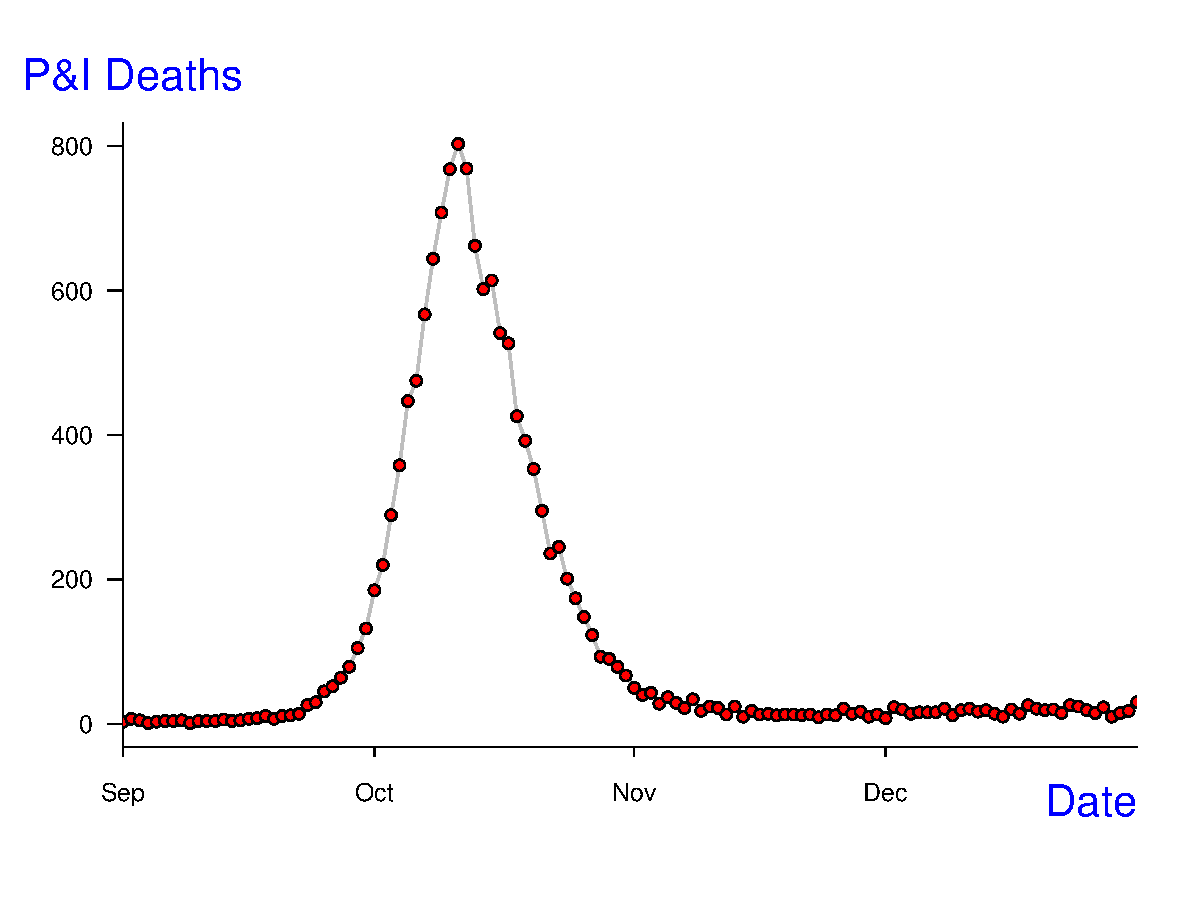
\includegraphics[width=\maxwidth]{figure/PnI_fig-1} 

\end{knitrout}
  }
  \end{proof}
  }

\PhilaDataReproduceB

\end{enumerate}

\section{Estimate $\R_0$ from the Philadelphia P\&I time series}

\begin{enumerate}[(a)]

\item \EstimateRna

 {\color{blue} \begin{proof}[Solution]
 {\color{magenta}
 Let mortality be denoted by $M(t)$ and prevalence be denoted by $I(t)$. If we assume that both mortality and prevalence grow exponentially, then we can write
\begin{equation*}
\begin{aligned}
M(t) = a e^{bt}
\end{aligned}
\end{equation*}
and
\begin{equation*}
\begin{aligned}
I(t) = g e^{ht}
\end{aligned}
\end{equation*}
for some constants $a$, $b$, $g$, and $h$. Furthermore, if we assume that $I(t) = \eta M(t - \tau)$, for some $\eta$ and $\tau$, then we can write
\begin{equation*}
\begin{aligned}
g e^{ht} = I(t) = \eta M(t - \tau) = \eta a e^{b(t-\tau)}.
\end{aligned}
\end{equation*}
Then $g e^{ht} = \eta ae^{-\tau} e ^{bt}$, and
\begin{equation*}
\begin{aligned}
e^{(h-b)t} = \frac{\eta ae^{-\tau} }{g}.
\end{aligned}
\end{equation*}
Notice that the RHS of this equation is constant and thus forces $h - b = 0$. That is, $h=b$, and thus both $I(t)$ and $M(t)$ have the same exponential growth rate.
}
 \end{proof}
 }

\item \EstimateRnb

  {\color{blue} \begin{proof}[Solution]
  {\color{magenta}
  \leavevmode
\begin{knitrout}
\definecolor{shadecolor}{rgb}{0.969, 0.969, 0.969}\color{fgcolor}\begin{kframe}
\begin{alltt}
\hlkwd{library}\hlstd{(tidyverse)}
\hlkwd{library}\hlstd{(ggplot2);} \hlkwd{theme_set}\hlstd{(}\hlkwd{theme_bw}\hlstd{())}

\hlstd{philadata} \hlkwb{<-} \hlstd{philadata}  \hlopt
  \hlkwd{mutate}\hlstd{(}\hlkwc{day} \hlstd{=} \hlkwd{as.numeric}\hlstd{(date)} \hlopt{-} \hlkwd{min}\hlstd{(}\hlkwd{as.numeric}\hlstd{(philadata}\hlopt{$}\hlstd{date)))}
\hlcom{#R stored dates as -18000 when numeric. transformed so first date sept 1918 is 0}
\hlstd{x} \hlkwb{<-} \hlstd{philadata} \hlopt
  \hlkwd{filter}\hlstd{(date} \hlopt{<=} \hlstr{"1918-10-7"} \hlopt{&} \hlstd{date} \hlopt{>=} \hlstr{"1918-09-15"}\hlstd{)}
\hlcom{#filter data in linear region}

\hlcom{#generate lm and give slope in base e}
\hlstd{lm.base.e} \hlkwb{<-} \hlkwd{lm}\hlstd{(}\hlkwd{log}\hlstd{(pim)}\hlopt{~}\hlstd{day,} \hlkwc{data}\hlstd{= x)}

\hlcom{#add column to x data with pts expected by our model above:}
\hlstd{x} \hlkwb{<-} \hlstd{x} \hlopt
  \hlkwd{mutate}\hlstd{(}\hlkwc{expected}\hlstd{=} \hlkwd{exp}\hlstd{(lm.base.e}\hlopt{$}\hlstd{coefficients[}\hlnum{1}\hlstd{])}\hlopt{*}
             \hlkwd{exp}\hlstd{(lm.base.e}\hlopt{$}\hlstd{coefficients[}\hlnum{2}\hlstd{]}\hlopt{*}\hlstd{day))}

\hlcom{#plot on log scale:}
\hlkwd{ggplot}\hlstd{(philadata,} \hlkwd{aes}\hlstd{(}\hlkwc{x}\hlstd{=date,} \hlkwc{y}\hlstd{=}\hlkwd{log}\hlstd{(pim)))} \hlopt{+}
  \hlkwd{geom_point}\hlstd{()} \hlopt{+}
  \hlkwd{annotate}\hlstd{(}\hlkwc{geom}\hlstd{=}\hlstr{"rect"}\hlstd{,} \hlkwc{xmin} \hlstd{=} \hlkwd{as.Date}\hlstd{(}\hlstr{"1918-10-7"}\hlstd{),}
           \hlkwc{xmax} \hlstd{=} \hlkwd{as.Date}\hlstd{(}\hlstr{"1918-09-15"}\hlstd{),} \hlkwc{ymin} \hlstd{=}\hlnum{0}\hlstd{,} \hlkwc{ymax}\hlstd{=}\hlnum{Inf}\hlstd{,}
           \hlkwc{alpha}\hlstd{=}\hlnum{0.2}\hlstd{)} \hlopt{+}
  \hlkwd{labs}\hlstd{(}\hlkwc{x}\hlstd{=}\hlstr{"Date"}\hlstd{,} \hlkwc{y}\hlstd{=}\hlstr{"log(P&I Mortality)"}\hlstd{)} \hlopt{+}
  \hlkwd{geom_line}\hlstd{(}\hlkwc{data}\hlstd{=x,} \hlkwd{aes}\hlstd{(}\hlkwc{x}\hlstd{=date,} \hlkwc{y}\hlstd{=}\hlkwd{log}\hlstd{(expected)),} \hlkwc{color}\hlstd{=}\hlstr{"tomato3"}\hlstd{)}
\end{alltt}
\end{kframe}
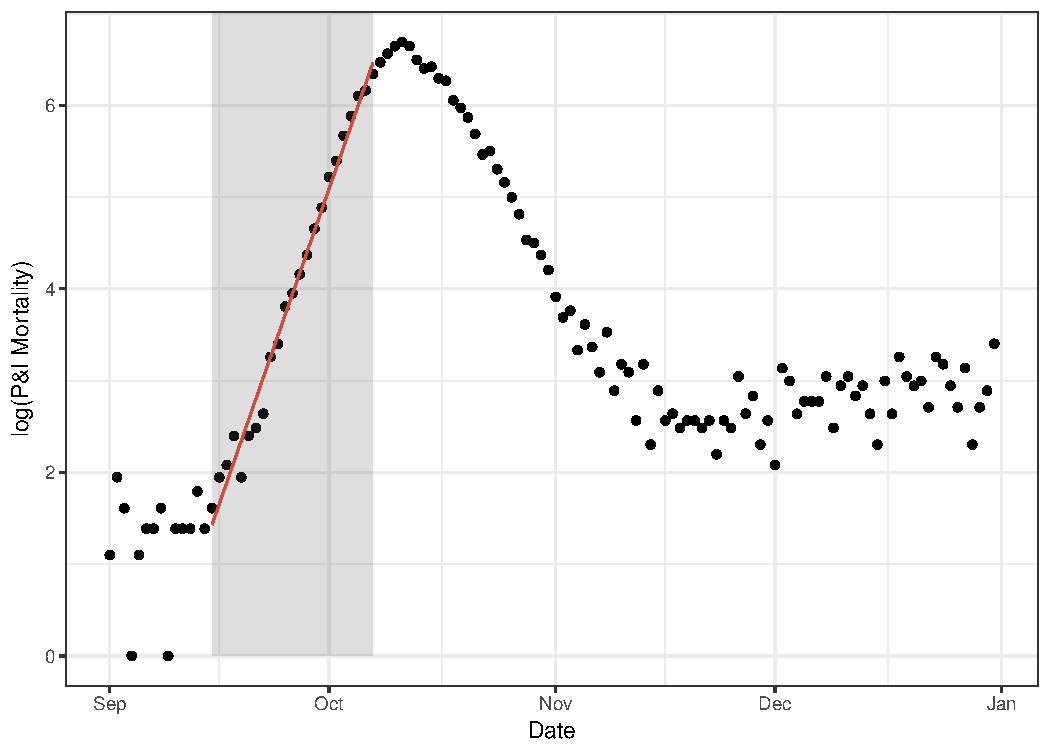
\includegraphics[width=\maxwidth]{figure/estimaternb-1} 
\begin{kframe}\begin{alltt}
\hlcom{#plot on normal scale and show how model fits:}
\hlkwd{ggplot}\hlstd{(philadata,} \hlkwd{aes}\hlstd{(}\hlkwc{x}\hlstd{=date,} \hlkwc{y}\hlstd{=pim))} \hlopt{+}
  \hlkwd{geom_point}\hlstd{()} \hlopt{+}
  \hlkwd{annotate}\hlstd{(}\hlkwc{geom}\hlstd{=}\hlstr{"rect"}\hlstd{,} \hlkwc{xmin} \hlstd{=} \hlkwd{as.Date}\hlstd{(}\hlstr{"1918-10-7"}\hlstd{),}
           \hlkwc{xmax} \hlstd{=} \hlkwd{as.Date}\hlstd{(}\hlstr{"1918-09-15"}\hlstd{),} \hlkwc{ymin} \hlstd{=}\hlnum{0}\hlstd{,} \hlkwc{ymax}\hlstd{=}\hlnum{Inf}\hlstd{,}
           \hlkwc{alpha}\hlstd{=}\hlnum{0.2}\hlstd{)} \hlopt{+}
  \hlkwd{labs}\hlstd{(}\hlkwc{x}\hlstd{=}\hlstr{"Date"}\hlstd{,} \hlkwc{y}\hlstd{=}\hlstr{"P&I Mortality"}\hlstd{)} \hlopt{+}
  \hlkwd{geom_line}\hlstd{(}\hlkwc{data}\hlstd{=x,} \hlkwd{aes}\hlstd{(}\hlkwc{x}\hlstd{=date,} \hlkwc{y}\hlstd{=expected),} \hlkwc{color}\hlstd{=}\hlstr{"tomato3"}\hlstd{)}
\end{alltt}
\end{kframe}
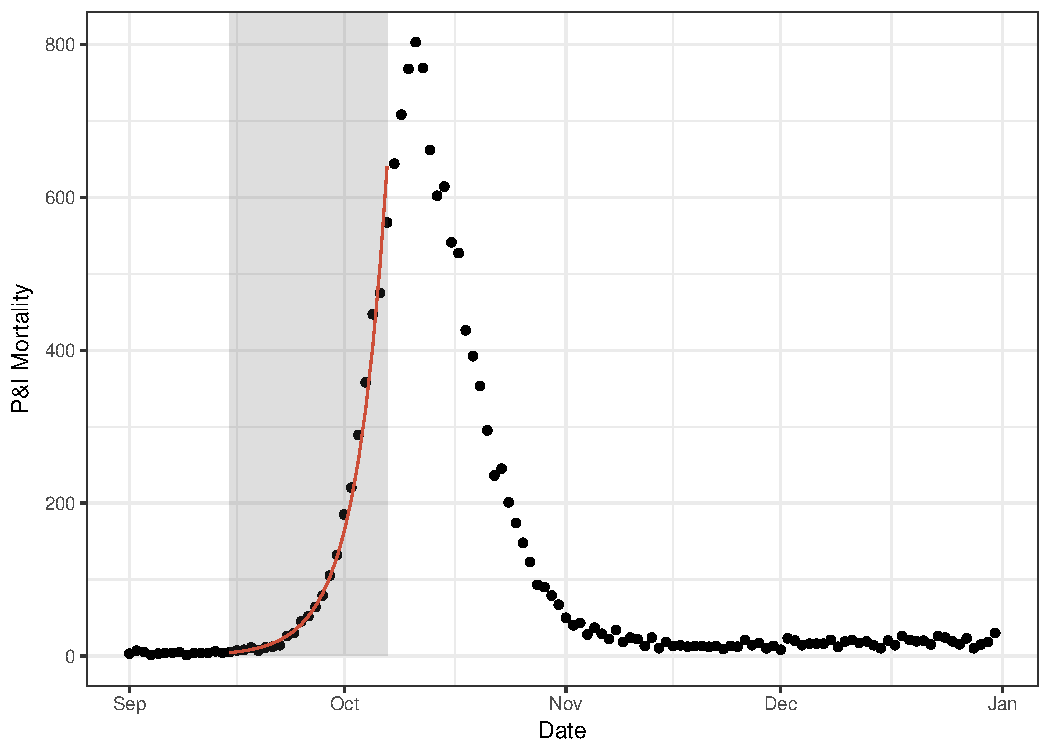
\includegraphics[width=\maxwidth]{figure/estimaternb-2} 

\end{knitrout}

To determine coefficients, we restricted the data to the portion in which the semi-log plot looks approximately linear, and fit a linear model using the \texttt{lm()} function to the log-transformed data. The slope and intercept of this fit is given below.

\begin{center}
\begin{tabular}{c c}\\
 slope & intercept \\
 \hline
 0.2286857 & -1.7714926
\end{tabular}
\end{center}
  
  
  }
  \end{proof}
  }
  
\item \EstimateRnc

  {\color{blue} \begin{proof}[Solution]
  {\color{magenta}
  We recall that the SIR model is given by Equation \ref{eq:SIRmodel}.
\begin{equation}
\label{eq:SIRmodel}
\begin{aligned}
\frac{dS}{dt}&=-\beta SI \\
\frac{dI}{dt}&=\beta SI - \gamma I \\
\frac{dR}{dt}&=\gamma I 
\end{aligned}
\end{equation}
Given that we are examining data that starts when $I$ is small (and then we have a constant exponential growth rate of 0.2287), we can use the assumption that $S\simeq 1$. Thus, this yields the equation $\frac{dI}{dt}\simeq\beta I - \gamma I$. Solving this, we have Equation \ref{eq:Isolve}
\begin{equation}
\label{eq:Isolve}
I=ce^{(\beta - \gamma)t}
\end{equation}
Following from the answer in Question 2 Part a, we know that the slope of 0.2287 of our fitted mortality curve in Part b is equal to the $\beta - \gamma$ slope we would have if we took the log of Equation \ref{eq:Isolve}.

We recall from the SIR model that the constant $\R_0$ is given by the product of the transmission rate and the mean infection period. Equivalently, we have that $\R_0 = \frac{\beta}{\gamma}$. Thus, in order to establish a value for $\R_0$, we need either $\gamma$ or $\beta$, as then we can solve for the other variable using that $\beta - \gamma = 0.2287$. It is much more logical to look for an independent measure of $\gamma$, as the mean infectious period given by $\frac{1}{\gamma}$ is easier to infer from data than the transmission rate. 

If in our case, the mean infectious period ($\frac{1}{\gamma}$) is 4 days, then we know that $\gamma = \frac{1}{4}$. Thus, we have that $\beta=0.4787$. From this information, we can solve for $\R_0 = 0.4787*4 = 1.9148$.
  }
  \end{proof}
  }

\end{enumerate}

\section{Fit the basic SIR model to the Philadelphia P\&I time series}

\begin{enumerate}[(a)]

\item \FitSIRa

\item \FitSIRbIntro
\begin{itemize}
    \item Your code will first need to load the \code{deSolve} package:
\begin{knitrout}
\definecolor{shadecolor}{rgb}{0.969, 0.969, 0.969}\color{fgcolor}\begin{kframe}
\begin{alltt}
\hlkwd{library}\hlstd{(deSolve)}
\end{alltt}
\end{kframe}
\end{knitrout}
    \item \FitSIRbii
\begin{knitrout}
\definecolor{shadecolor}{rgb}{0.969, 0.969, 0.969}\color{fgcolor}\begin{kframe}
\begin{alltt}
\hlstd{plot.sine} \hlkwb{<-} \hlkwa{function}\hlstd{(} \hlkwc{xmin}\hlstd{=}\hlnum{0}\hlstd{,} \hlkwc{xmax}\hlstd{=}\hlnum{2}\hlopt{*}\hlstd{pi ) \{}
  \hlstd{x} \hlkwb{<-} \hlkwd{seq}\hlstd{(xmin,xmax,}\hlkwc{length}\hlstd{=}\hlnum{100}\hlstd{)}
  \hlkwd{plot}\hlstd{(x,} \hlkwd{sin}\hlstd{(x),} \hlkwc{typ}\hlstd{=}\hlstr{"l"}\hlstd{)}
  \hlkwd{grid}\hlstd{()} \hlcom{# add a light grey grid}
\hlstd{\}}
\hlkwd{plot.sine}\hlstd{(}\hlkwc{xmax}\hlstd{=}\hlnum{4}\hlopt{*}\hlstd{pi)}
\end{alltt}
\end{kframe}
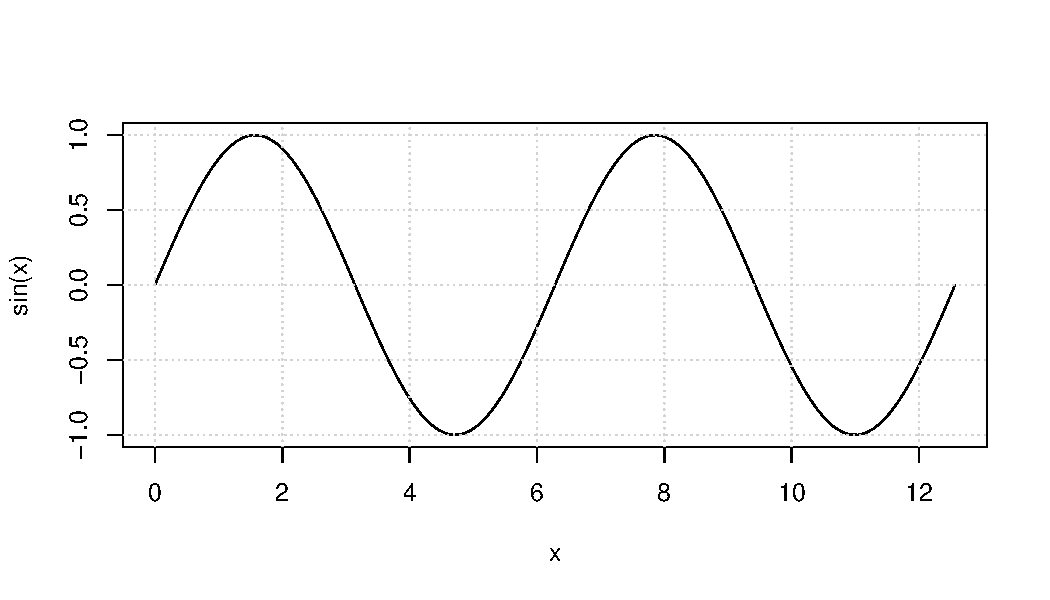
\includegraphics[width=\maxwidth]{figure/plot_sine-1} 

\end{knitrout}
  \item \FitSIRbiiiA
\begin{knitrout}
\definecolor{shadecolor}{rgb}{0.969, 0.969, 0.969}\color{fgcolor}\begin{kframe}
\begin{alltt}
\hlcom{## Vector Field for SI model}
\hlstd{SI.vector.field} \hlkwb{<-} \hlkwa{function}\hlstd{(}\hlkwc{t}\hlstd{,} \hlkwc{vars}\hlstd{,} \hlkwc{parms}\hlstd{=}\hlkwd{c}\hlstd{(}\hlkwc{beta}\hlstd{=}\hlnum{2}\hlstd{,}\hlkwc{gamma}\hlstd{=}\hlnum{1}\hlstd{)) \{}
  \hlkwd{with}\hlstd{(}\hlkwd{as.list}\hlstd{(}\hlkwd{c}\hlstd{(parms, vars)), \{}
    \hlstd{dx} \hlkwb{<-} \hlopt{-}\hlstd{beta}\hlopt{*}\hlstd{x}\hlopt{*}\hlstd{y} \hlcom{# dS/dt}
    \hlstd{dy} \hlkwb{<-} \hlstd{beta}\hlopt{*}\hlstd{x}\hlopt{*}\hlstd{y}  \hlcom{# dI/dt}
    \hlstd{vec.fld} \hlkwb{<-} \hlkwd{c}\hlstd{(}\hlkwc{dx}\hlstd{=dx,} \hlkwc{dy}\hlstd{=dy)}
    \hlkwd{return}\hlstd{(}\hlkwd{list}\hlstd{(vec.fld))} \hlcom{# ode() requires a list}
  \hlstd{\})}
\hlstd{\}}
\end{alltt}
\end{kframe}
\end{knitrout}

\FitSIRbiiiB
\begin{knitrout}
\definecolor{shadecolor}{rgb}{0.969, 0.969, 0.969}\color{fgcolor}\begin{kframe}
\begin{alltt}
\hlcom{## Draw solution}
\hlstd{draw.soln} \hlkwb{<-} \hlkwa{function}\hlstd{(}\hlkwc{ic}\hlstd{=}\hlkwd{c}\hlstd{(}\hlkwc{x}\hlstd{=}\hlnum{1}\hlstd{,}\hlkwc{y}\hlstd{=}\hlnum{0}\hlstd{),} \hlkwc{tmax}\hlstd{=}\hlnum{1}\hlstd{,}
                      \hlkwc{times}\hlstd{=}\hlkwd{seq}\hlstd{(}\hlnum{0}\hlstd{,tmax,}\hlkwc{by}\hlstd{=tmax}\hlopt{/}\hlnum{500}\hlstd{),}
                      \hlkwc{func}\hlstd{,} \hlkwc{parms}\hlstd{,}
                      \hlkwc{col}\hlstd{=}\hlstr{"blue"}\hlstd{,}
                      \hlkwc{...} \hlstd{) \{}
  \hlstd{soln} \hlkwb{<-} \hlkwd{ode}\hlstd{(ic, times, func, parms)}
  \hlkwd{lines}\hlstd{(times, soln[,}\hlstr{"y"}\hlstd{],} \hlkwc{col}\hlstd{=col,} \hlkwc{lwd}\hlstd{=}\hlnum{3}\hlstd{, ... )}
\hlstd{\}}
\end{alltt}
\end{kframe}
\end{knitrout}
\FitSIRbiiiC
\begin{knitrout}
\definecolor{shadecolor}{rgb}{0.969, 0.969, 0.969}\color{fgcolor}\begin{kframe}
\begin{alltt}
\hlstd{soln} \hlkwb{<-} \hlkwd{ode}\hlstd{(}\hlkwc{times}\hlstd{=times,} \hlkwc{func}\hlstd{=func,} \hlkwc{parms}\hlstd{=parms,} \hlkwc{y}\hlstd{=ic)}
\end{alltt}
\end{kframe}
\end{knitrout}

We can now use our \code{draw.soln()} function to plot a few solutions of the SI model.

\begin{knitrout}
\definecolor{shadecolor}{rgb}{0.969, 0.969, 0.969}\color{fgcolor}\begin{kframe}
\begin{alltt}
\hlcom{## Plot solutions of the SI model}
\hlstd{tmax} \hlkwb{<-} \hlnum{10} \hlcom{# end time for numerical integration of the ODE}
\hlcom{## draw box for plot:}
\hlkwd{plot}\hlstd{(}\hlnum{0}\hlstd{,}\hlnum{0}\hlstd{,}\hlkwc{xlim}\hlstd{=}\hlkwd{c}\hlstd{(}\hlnum{0}\hlstd{,tmax),}\hlkwc{ylim}\hlstd{=}\hlkwd{c}\hlstd{(}\hlnum{0}\hlstd{,}\hlnum{1}\hlstd{),}
     \hlkwc{type}\hlstd{=}\hlstr{"n"}\hlstd{,}\hlkwc{xlab}\hlstd{=}\hlstr{"Time (t)"}\hlstd{,}\hlkwc{ylab}\hlstd{=}\hlstr{"Prevalence (I)"}\hlstd{,}\hlkwc{las}\hlstd{=}\hlnum{1}\hlstd{)}
\hlcom{## initial conditions:}
\hlstd{I0} \hlkwb{<-} \hlnum{0.001}
\hlstd{S0} \hlkwb{<-} \hlnum{1} \hlopt{-} \hlstd{I0}
\hlcom{## draw solutions for several values of parameter beta:}
\hlstd{betavals} \hlkwb{<-} \hlkwd{c}\hlstd{(}\hlnum{1.5}\hlstd{,}\hlnum{2}\hlstd{,}\hlnum{2.5}\hlstd{)}
\hlkwa{for} \hlstd{(i} \hlkwa{in} \hlnum{1}\hlopt{:}\hlkwd{length}\hlstd{(betavals)) \{}
  \hlkwd{draw.soln}\hlstd{(}\hlkwc{ic}\hlstd{=}\hlkwd{c}\hlstd{(}\hlkwc{x}\hlstd{=S0,}\hlkwc{y}\hlstd{=I0),} \hlkwc{tmax}\hlstd{=tmax,}
            \hlkwc{func}\hlstd{=SI.vector.field,}
            \hlkwc{parms}\hlstd{=}\hlkwd{c}\hlstd{(}\hlkwc{beta}\hlstd{=betavals[i],}\hlkwc{gamma}\hlstd{=}\hlnum{1}\hlstd{),}
            \hlkwc{lty}\hlstd{=i} \hlcom{# use a different line style for each solution}
            \hlstd{)}
\hlstd{\}}
\end{alltt}
\end{kframe}
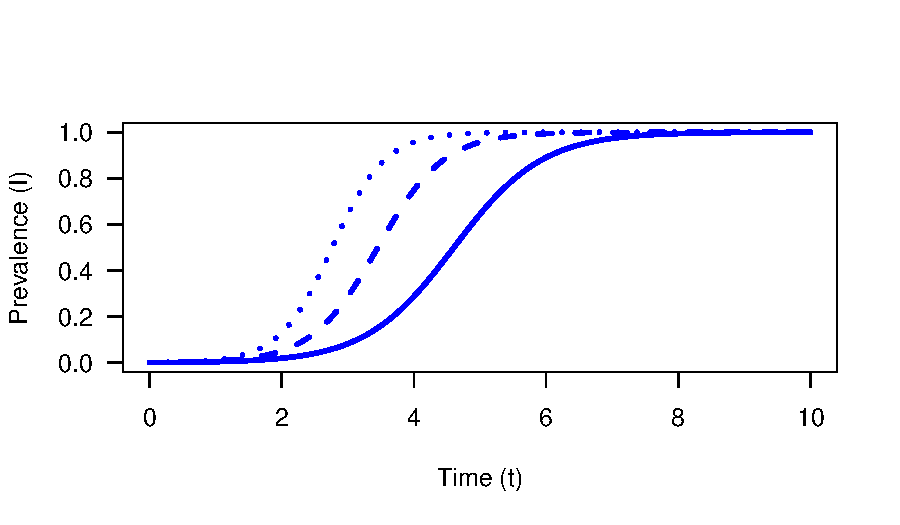
\includegraphics[width=\maxwidth]{figure/plot_SI_model-1} 

\end{knitrout}


  \end{itemize}
 
 {\color{blue} \begin{proof}[Solution]
 {\color{magenta}
First, we must determine values for $\beta$ and $\gamma$, since the basic SIR model that we have studied in class has parameters $\beta$ and $\gamma$.
We can do so by following the method described in problem 2 (c). We observe that $\gamma$ is the reciprocal of the infectious period, and that $\beta = \R_0 \gamma$.
If we suppose that $I_0 = 10^{-3}$ and $S_0 = 1 - I_0$, we can follow the template given in the question to graph solutions for a mean infectious period of 4 days, and for various $\mathcal{R}_0$ values. 
We begin by defining a vector field for the SIR model:
\begin{knitrout}
\definecolor{shadecolor}{rgb}{0.969, 0.969, 0.969}\color{fgcolor}\begin{kframe}
\begin{alltt}
\hlcom{## Vector Field for SIR model}
\hlstd{SIR.vector.field} \hlkwb{<-} \hlkwa{function}\hlstd{(}\hlkwc{t}\hlstd{,} \hlkwc{vars}\hlstd{,} \hlkwc{parms}\hlstd{=}\hlkwd{c}\hlstd{(}\hlkwc{beta}\hlstd{=}\hlnum{2}\hlstd{,}\hlkwc{gamma}\hlstd{=}\hlnum{1}\hlstd{)) \{}
    \hlkwd{with}\hlstd{(}\hlkwd{as.list}\hlstd{(}\hlkwd{c}\hlstd{(parms, vars)), \{}
        \hlstd{inf} \hlkwb{<-} \hlstd{beta}\hlopt{*}\hlstd{x}\hlopt{*}\hlstd{y} \hlcom{## infection}
        \hlkwd{return}\hlstd{(}\hlkwd{list}\hlstd{(}\hlkwd{c}\hlstd{(}\hlkwc{dx}\hlstd{=}\hlopt{-}\hlstd{inf,} \hlkwc{dy}\hlstd{=inf}\hlopt{-}\hlstd{gamma}\hlopt{*}\hlstd{y)))}
    \hlstd{\})}
\hlstd{\}}
\end{alltt}
\end{kframe}
\end{knitrout}

Then, we can define a function that draws the solution to the SIR model given parameters, initial values, and the maximum time step:
\begin{knitrout}
\definecolor{shadecolor}{rgb}{0.969, 0.969, 0.969}\color{fgcolor}\begin{kframe}
\begin{alltt}
\hlstd{draw.sir} \hlkwb{<-} \hlkwa{function}\hlstd{(}\hlkwc{S0}\hlstd{,}
                     \hlkwc{I0}\hlstd{,}
                     \hlkwc{R0}\hlstd{,}
                     \hlkwc{inf.period}\hlstd{,}
                     \hlkwc{tmax}\hlstd{,} \hlcom{## max time}
                     \hlkwc{...}\hlstd{) \{}
    \hlcom{## draw solution curve (prevalence)}
    \hlkwd{draw.soln}\hlstd{(}\hlkwc{ic}\hlstd{=}\hlkwd{c}\hlstd{(}\hlkwc{x}\hlstd{=S0,} \hlkwc{y}\hlstd{=I0),}
              \hlkwc{tmax}\hlstd{=tmax,}
              \hlkwc{func}\hlstd{=SIR.vector.field,}
              \hlkwc{parms}\hlstd{=}\hlkwd{c}\hlstd{(}\hlkwc{beta}\hlstd{=R0}\hlopt{/}\hlstd{inf.period,}
                      \hlkwc{gamma}\hlstd{=}\hlnum{1}\hlopt{/}\hlstd{inf.period),}
              \hlstd{...)}
\hlstd{\}}
\end{alltt}
\end{kframe}
\end{knitrout}

 }
 \end{proof}
 }

\item \FitSIRc

  {\color{blue} \begin{proof}[Solution]
  {\color{magenta}
\begin{knitrout}
\definecolor{shadecolor}{rgb}{0.969, 0.969, 0.969}\color{fgcolor}\begin{kframe}
\begin{alltt}
\hlcom{## setting up initial conditions}
\hlcom{## as well as parameters}
\hlstd{I0} \hlkwb{<-} \hlnum{1e-3}
\hlstd{S0} \hlkwb{<-} \hlnum{1} \hlopt{-} \hlstd{I0}
\hlstd{inf.period} \hlkwb{<-} \hlnum{4}
\hlstd{R0} \hlkwb{<-} \hlkwd{c}\hlstd{(}\hlnum{1.2}\hlstd{,} \hlnum{1.5}\hlstd{,} \hlnum{1.8}\hlstd{,} \hlnum{2}\hlstd{,} \hlnum{3}\hlstd{,} \hlnum{4}\hlstd{)}
\hlstd{n} \hlkwb{<-} \hlkwd{length}\hlstd{(R0)}
\hlstd{tmax} \hlkwb{<-} \hlnum{150}

\hlcom{## set up plot window}
\hlkwd{plot}\hlstd{(}\hlnum{NA}\hlstd{,} \hlkwc{xlim}\hlstd{=}\hlkwd{c}\hlstd{(}\hlnum{0}\hlstd{,tmax),} \hlkwc{ylim}\hlstd{=}\hlkwd{c}\hlstd{(}\hlnum{0}\hlstd{,}\hlnum{0.4}\hlstd{),}
     \hlkwc{xlab}\hlstd{=}\hlstr{"Time (days)"}\hlstd{,} \hlkwc{ylab}\hlstd{=}\hlstr{"Prevalence"}\hlstd{)}
\hlcom{## actually plot curves}
\hlcom{## Map is a fancy way of avoiding loops}
\hlstd{SIR.plot} \hlkwb{<-} \hlkwd{Map}\hlstd{(draw.sir,} \hlkwc{S0}\hlstd{=S0,} \hlkwc{I0}\hlstd{=I0,} \hlkwc{R0}\hlstd{=R0,} \hlkwc{inf.period}\hlstd{=inf.period,}
    \hlkwc{lty}\hlstd{=}\hlnum{1}\hlopt{:}\hlstd{n,} \hlkwc{col}\hlstd{=}\hlnum{1}\hlopt{:}\hlstd{n,}
    \hlkwc{tmax}\hlstd{=tmax}
\hlstd{)}

\hlkwd{legend}\hlstd{(}
    \hlkwc{x}\hlstd{=}\hlnum{90}\hlstd{,} \hlkwc{y}\hlstd{=}\hlnum{0.4}\hlstd{,}
    \hlkwc{legend}\hlstd{=R0,} \hlkwc{lty}\hlstd{=}\hlnum{1}\hlopt{:}\hlstd{n,} \hlkwc{col}\hlstd{=}\hlnum{1}\hlopt{:}\hlstd{n,}
    \hlkwc{lwd}\hlstd{=}\hlnum{3}\hlstd{,} \hlkwc{title}\hlstd{=}\hlstr{"Reproductive number"}\hlstd{,} \hlkwc{seg.len}\hlstd{=}\hlnum{5}
\hlstd{)}
\end{alltt}
\end{kframe}
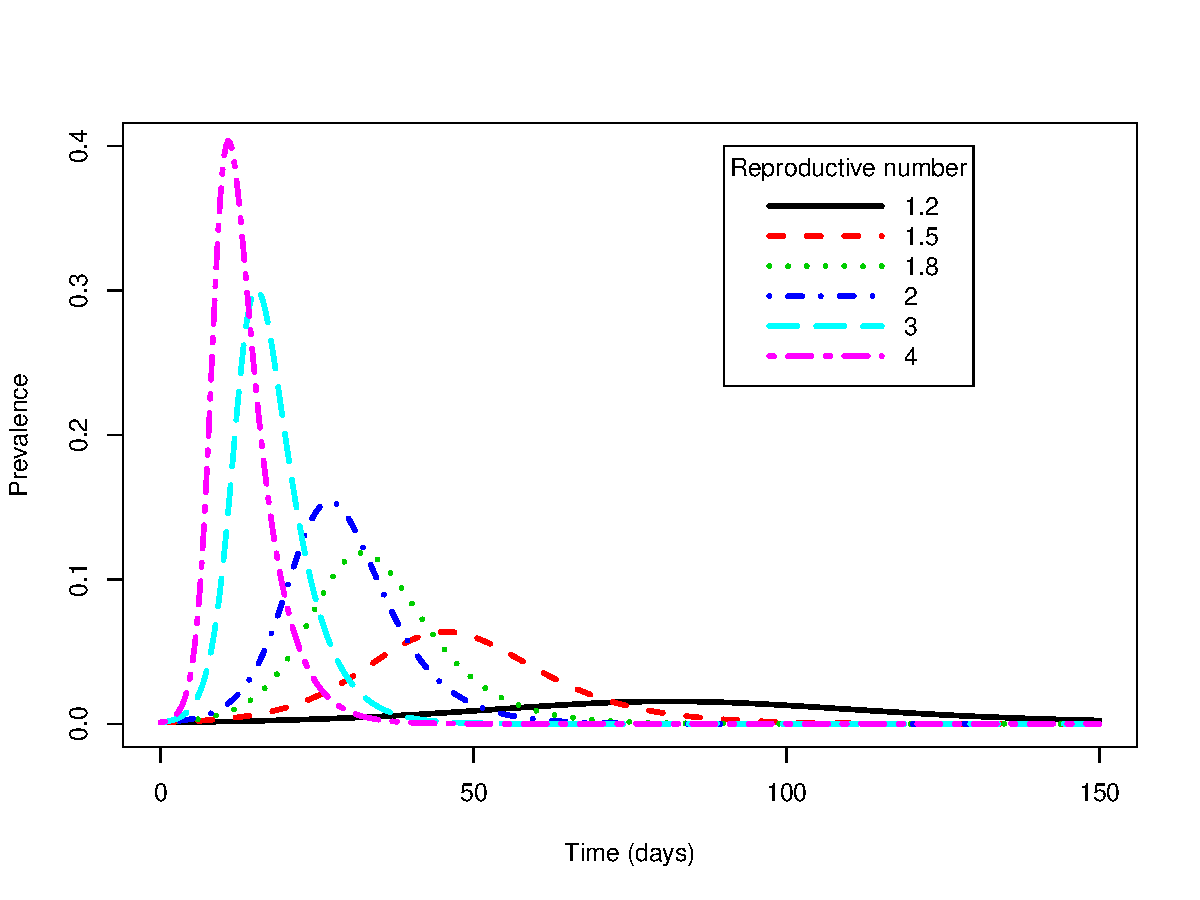
\includegraphics[width=\maxwidth]{figure/sir_plot-1} 

\end{knitrout}
  }
  \end{proof}
  }
  
\item \FitSIRd

  {\color{blue} \begin{proof}[Solution]
  {\color{magenta}
In section 2 (a), it was assumed that mortality and prevalence have the following relationship:
$$
I(t) = \eta M(t-\tau).
$$
Rearranging, we have
$$
M(t) = \frac{1}{\eta} I(t+\tau)
$$
So we will have to run the model for $t+\tau$ time steps to compare and estimate $\eta$, $\tau$, $S(0)$, $I(0)$, $\R_0$, and infectious period.

Here is the function that will return a data frame whose columns are date and expected daily moratlity, given parameters and initial conditions:
\begin{knitrout}
\definecolor{shadecolor}{rgb}{0.969, 0.969, 0.969}\color{fgcolor}\begin{kframe}
\begin{alltt}
\hlstd{simulate_mortality} \hlkwb{<-} \hlkwa{function}\hlstd{(}\hlkwc{S0}\hlstd{,}
                               \hlkwc{I0}\hlstd{,}
                               \hlkwc{R0}\hlstd{,}
                               \hlkwc{inf.period}\hlstd{,}
                               \hlkwc{eta}\hlstd{,}
                               \hlkwc{tau}\hlstd{,}
                               \hlkwc{tmax}\hlstd{=}\hlkwd{nrow}\hlstd{(philadata)) \{}
    \hlcom{## first we want to solve ode}
    \hlstd{soln} \hlkwb{<-} \hlkwd{as.data.frame}\hlstd{(}\hlkwd{ode}\hlstd{(}
        \hlkwc{y}\hlstd{=}\hlkwd{c}\hlstd{(}\hlkwc{x}\hlstd{=S0,} \hlkwc{y}\hlstd{=I0),}
        \hlkwc{times}\hlstd{=}\hlnum{1}\hlopt{:}\hlstd{(tmax}\hlopt{+}\hlstd{tau),}
        \hlkwc{func}\hlstd{=SIR.vector.field,}
        \hlkwc{parms}\hlstd{=}\hlkwd{c}\hlstd{(}\hlkwc{beta}\hlstd{=R0}\hlopt{/}\hlstd{inf.period,}
                      \hlkwc{gamma}\hlstd{=}\hlnum{1}\hlopt{/}\hlstd{inf.period)))}

    \hlcom{## then mortality is approximation}
    \hlkwd{data.frame}\hlstd{(}
        \hlkwc{date}\hlstd{=philadata}\hlopt{$}\hlstd{date,}
        \hlkwc{pim}\hlstd{=}\hlkwd{tail}\hlstd{(soln}\hlopt{$}\hlstd{y,} \hlopt{-}\hlstd{tau)}\hlopt{/}\hlstd{eta}
    \hlstd{)}
\hlstd{\}}
\end{alltt}
\end{kframe}
\end{knitrout}

Now here is the estimate that we found via trial and error:
$$
S(0)=1-10^{-7}, I(0)=10^{-7}, \R_0=2.2, \frac{1}{\gamma}=4, \eta = 0.00025, \tau=14.
$$
Then, we can compare our estimated mortality curve with the given data:
\begin{knitrout}
\definecolor{shadecolor}{rgb}{0.969, 0.969, 0.969}\color{fgcolor}\begin{kframe}
\begin{alltt}
\hlcom{## simulating mortality using parameters we estimated}
\hlstd{mfit} \hlkwb{<-} \hlkwd{simulate_mortality}\hlstd{(}\hlkwc{S0}\hlstd{=}\hlnum{1}\hlopt{-}\hlnum{1e-7}\hlstd{,} \hlkwc{I0}\hlstd{=}\hlnum{1e-7}\hlstd{,}
                           \hlkwc{R0}\hlstd{=}\hlnum{2.2}\hlstd{,} \hlkwc{inf.period} \hlstd{=} \hlnum{4}\hlstd{,}
                           \hlkwc{eta}\hlstd{=}\hlnum{0.00025}\hlstd{,} \hlkwc{tau}\hlstd{=}\hlnum{14}\hlstd{)}

\hlcom{## plotting expected mortality curve}
\hlkwd{plot}\hlstd{(mfit,} \hlkwc{type}\hlstd{=}\hlstr{"l"}\hlstd{,} \hlkwc{lwd}\hlstd{=}\hlnum{3}\hlstd{,} \hlkwc{col}\hlstd{=}\hlstr{"blue"}\hlstd{,} \hlkwc{ylim}\hlstd{=}\hlkwd{c}\hlstd{(}\hlnum{0}\hlstd{,}\hlnum{800}\hlstd{))}
\hlkwd{points}\hlstd{(philadata)}
\hlkwd{legend}\hlstd{(}
    \hlstr{"topright"}\hlstd{,}
    \hlkwc{legend}\hlstd{=}\hlkwd{c}\hlstd{(}\hlstr{"data"}\hlstd{,} \hlstr{"fit"}\hlstd{),}
    \hlkwc{lty}\hlstd{=}\hlkwd{c}\hlstd{(}\hlnum{NA}\hlstd{,} \hlnum{1}\hlstd{),}
    \hlkwc{pch}\hlstd{=}\hlkwd{c}\hlstd{(}\hlnum{1}\hlstd{,} \hlnum{NA}\hlstd{),}
    \hlkwc{col}\hlstd{=}\hlkwd{c}\hlstd{(}\hlstr{"black"}\hlstd{,} \hlstr{"blue"}\hlstd{),}
    \hlkwc{lwd}\hlstd{=}\hlnum{2}
\hlstd{)}
\end{alltt}
\end{kframe}
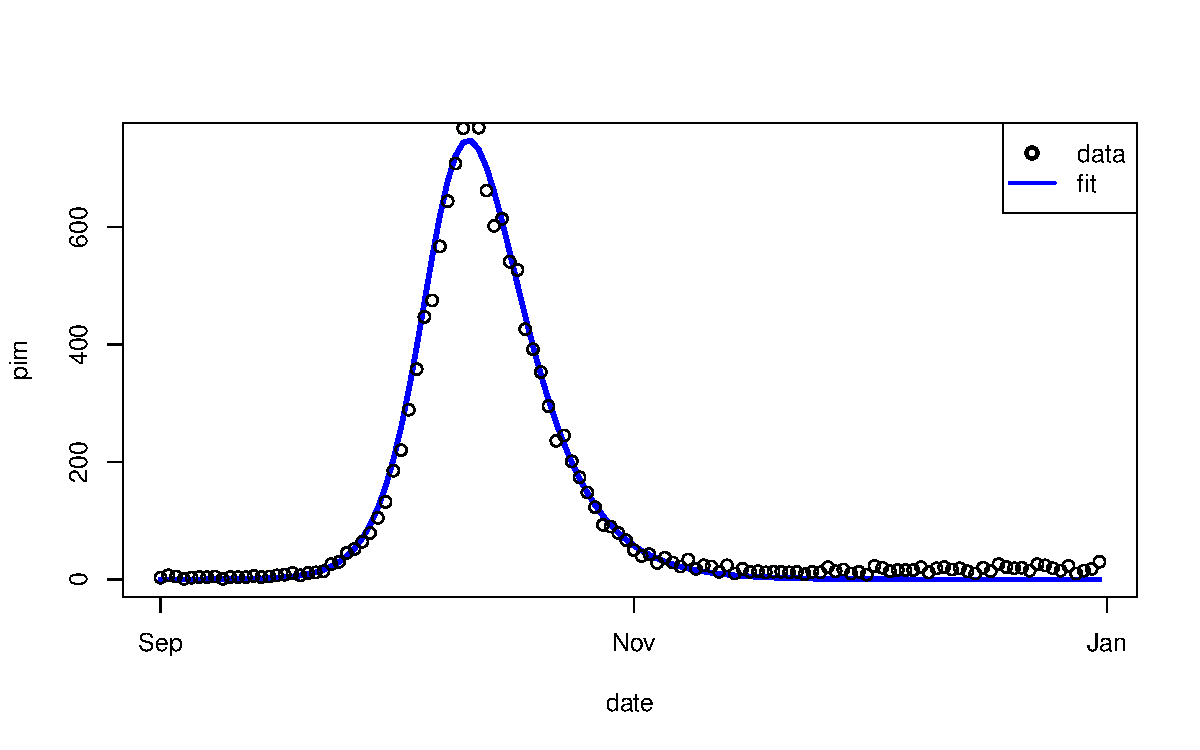
\includegraphics[width=\maxwidth]{figure/phila_fit-1} 

\end{knitrout}
Note that our fit appears to underestimate mortality after November. We can take a closer look at the difference by plotting the graph on a log scale:
\begin{knitrout}
\definecolor{shadecolor}{rgb}{0.969, 0.969, 0.969}\color{fgcolor}\begin{kframe}
\begin{alltt}
\hlkwd{plot}\hlstd{(mfit,} \hlkwc{type}\hlstd{=}\hlstr{"l"}\hlstd{,} \hlkwc{lwd}\hlstd{=}\hlnum{3}\hlstd{,} \hlkwc{col}\hlstd{=}\hlstr{"blue"}\hlstd{,} \hlkwc{log}\hlstd{=}\hlstr{"y"}\hlstd{)}
\hlkwd{points}\hlstd{(philadata)}
\hlkwd{legend}\hlstd{(}
    \hlstr{"topright"}\hlstd{,}
    \hlkwc{legend}\hlstd{=}\hlkwd{c}\hlstd{(}\hlstr{"data"}\hlstd{,} \hlstr{"fit"}\hlstd{),}
    \hlkwc{lty}\hlstd{=}\hlkwd{c}\hlstd{(}\hlnum{NA}\hlstd{,} \hlnum{1}\hlstd{),}
    \hlkwc{pch}\hlstd{=}\hlkwd{c}\hlstd{(}\hlnum{1}\hlstd{,} \hlnum{NA}\hlstd{),}
    \hlkwc{col}\hlstd{=}\hlkwd{c}\hlstd{(}\hlstr{"black"}\hlstd{,} \hlstr{"blue"}\hlstd{),}
    \hlkwc{lwd}\hlstd{=}\hlnum{2}
\hlstd{)}
\end{alltt}
\end{kframe}
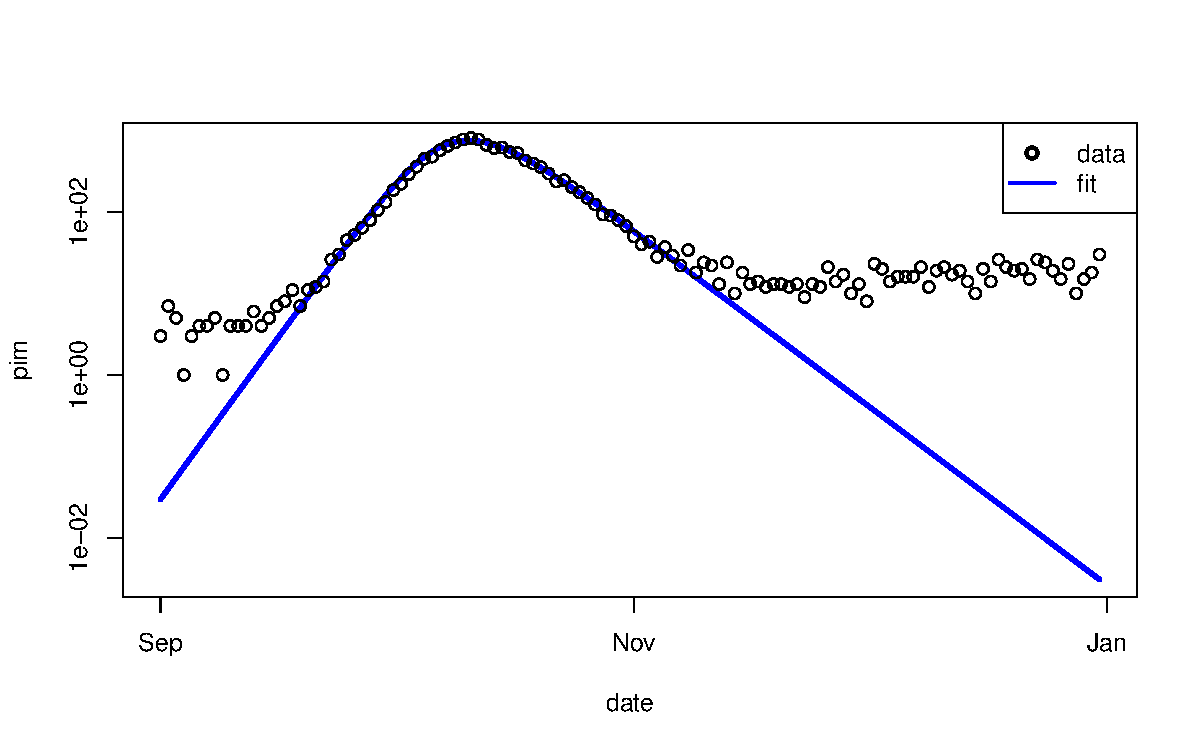
\includegraphics[width=\maxwidth]{figure/phila_fit_log-1} 

\end{knitrout}
Notice that we have a very good fit in the middle but not near the two opposite ends. The SIR model predicts that the disease will become extinct after a finite period of time. However, mortality data suggests that the epidemic will continue even after a long period of time. Hence, we can conlude that the SIR model might simply be insufficient to explain the data and will not fit very well even if we tried harder.
  }
  \end{proof}
  }
 
\end{enumerate}

\section{Executive summary for the Public Health Agency}

\ExecSumm
\newpage
The 1918 influenza pandemic was one of the worst influenza epidemics ever recorded. Data from this period are therefore valuable to study because they can provide insight into how similar present-day infectious diseases might spread in a population. In this report, we summarize results from the analysis of 1918 pneumonia and influenza mortality data in Philadelphia, and discuss potential implications for influenza dynamics and future outbreaks.

Using these data, we can characterize key features of the spread of this epidemic. We begin by analyzing the average number of secondary cases caused by a primary case. Knowing this quantity allows us to estimate the total number of infected individuals and to predict how many people would potentially be infected in any future flu epidemics. In particular, we observed that the average number of secondary cases caused by a primary case is linked to how fast an epidemic grows and how long an infection lasts. Hence, if we can estimate these quantities in the early stages of these epidemics, we will be able to better prepare for future epidemics.

For the 1918 flu, we estimate based on the Philadelphia data that a primary case of influenza would have caused approximately 1.9 to 2.3 secondary cases, assuming that the average flu infection lasts four days. From this, we estimate that about 76\%-86\% of the population would have been ultimately infected by this flu strain. Furthermore, we expect that at the peak of the epidemic, about 14\%-20\% of the population would have been infected simultaneously, meaning that current hospital capacities are unlikely to be able to handle a similar epidemic. In addition, if another flu of this magnitude were to occur, 47\%-56\% of the population would need to be vaccinated in order to prevent the disease from growing in the population. That is, if this portion of the population were vaccinated, we would expect the total number of simultaneously infected individuals in the population to decrease, thereby preventing an epidemic. 

The investigations performed so far were rather preliminary, and additional analysis would be beneficial. If the PHAC were to continue to fund research on historical flu epidemics, we would pursue additional avenues which could help increase the accuracy of our estimate of the average number of secondary cases caused by a primary case. This improved value would in turn provide more accurate information about final expected epidemic size. One possible way to improve the estimate would be to investigate external factors that might help us better explain the data in the 1918 time series. For example, after investigating the biological processes that the spread of influenza relies upon, we would introduce additional terms into our model to try to represent the disease dynamics in greater detail. Another possible way to improve our estimate of the average number of secondary cases caused by a primary case is through examining other time series from epidemics in different locations which were likely caused by the same strain of influenza. This would help us deduce if our model and estimated values are consistent with the dynamics of influenza in general.


\bigskip

\centerline{\bf--- END OF ASSIGNMENT ---}

\bigskip
Compile time for this document:
\today\ @ \thistime

\end{document}
